\documentclass[10pt]{beamer}

\beamertemplatenavigationsymbolsempty

\usepackage{booktabs}
\usepackage{colortbl}

\usepackage{tikz}
\usetikzlibrary{positioning,shapes.misc,calc,backgrounds,scopes} 
\tikzset{boxed/.style={
  thick,
  draw=black,
  top color=white,
  text height=1.5ex,
  text depth=.25ex
}}


\newcommand\lo{\ensuremath{\boldsymbol{-}}}
\newcommand\hi{\ensuremath{\boldsymbol{+}}}

\title{Response Surface Methodology:\\Central Composite Designs}
\author{BIOE 498/598 PJ}
\date{Spring 2022}

\begin{document}
\frame{\titlepage}

\begin{frame}{Surrogate Optimization}

\begin{center}
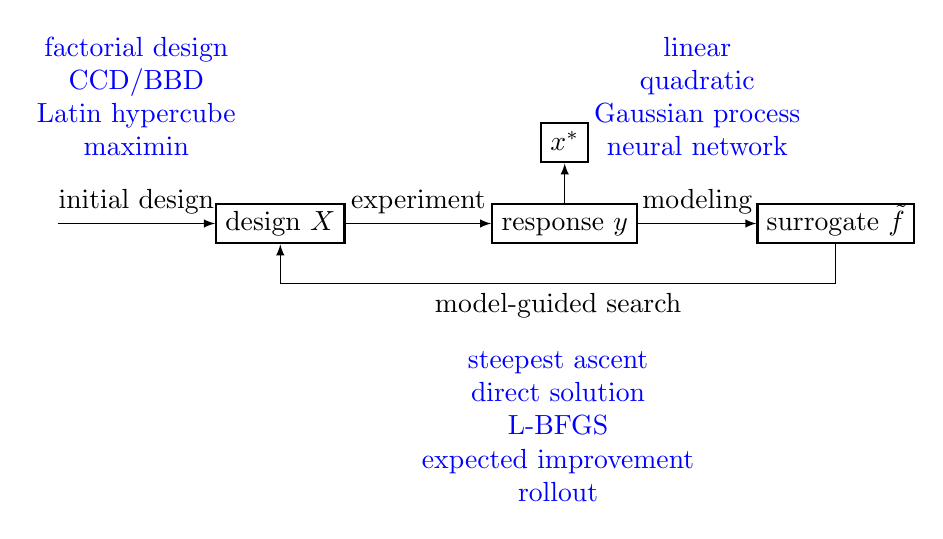
\begin{tikzpicture}[>=latex]
  \node (start) {};
  \node (data) [boxed, right=2cm of start] {design $X$};
  \node (response) [boxed,right=1.85cm of data] {response $y$};
  \node (optimal) [boxed,above=0.5cm of response] {$x^*$};
  \draw [->] (start) -- (data) node [midway,above] (initial) {initial design};
  \draw [->] (data) -- (response) node [midway,above] {experiment};
  \draw [->] (response) -- (optimal);
  \node (surrogate) [boxed,right=1.5cm of response] {surrogate $\tilde{f}$};
  \draw [->] (response) -- (surrogate) node [midway,above] (modeling) {modeling};
  \draw [->] (surrogate.south) -- ++(0,-0.5) -| (data.south) node [near start,below] (search) {model-guided search};
  \node [blue,align=center,above=0.5em of initial] {factorial design\\CCD/BBD\\Latin hypercube\\maximin};
  \node [blue,align=center,above=0.5em of modeling] {linear\\quadratic\\Gaussian process\\neural network};
  \node [blue,align=center,below=0.5em of search] {steepest ascent\\direct solution\\L-BFGS\\expected improvement\\rollout};
\end{tikzpicture}
\end{center}

\end{frame}

\newcommand<>\uncoverunderbrace[2]{%
  \onslide#3 \underbrace{ \onslide<1->%
  #1%
  \onslide#3 }_{#2} \onslide<1->%
}

\begin{frame}[shrink]{Approximating $f$ with a general quadratic}

Let's find the second-order Taylor series of $f(x_1,x_2)$ centered at zero:

{\small
	\begin{align*}
		f(x_1,x_2) \approx&\, 
		  \uncoverunderbrace<2->{f\rvert_0}{\beta_0} 
		  + \uncoverunderbrace<2->{\frac{\partial f}{\partial x_1}\bigg\rvert_0}{\beta_1}\!x_1 
		  + \uncoverunderbrace<2->{\frac{\partial f}{\partial x_2}\bigg\rvert_0}{\beta_2}x_2
		  + \uncoverunderbrace<2->{\frac{1}{2}\frac{\partial^2 f}{\partial x_1^2}\bigg\rvert_0}{\beta_{11}}x_1^2 
		  + \uncoverunderbrace<2->{\frac{1}{2}\frac{\partial^2 f}{\partial x_2^2}\bigg\rvert_0}{\beta_{22}}x_2^2
		  + \uncoverunderbrace<2->{\frac{1}{2}\frac{\partial^2 f}{\partial x_1\partial x_2}\bigg\rvert_0}{\beta_{12}}x_1x_2
	\end{align*}
	\onslide<3->{
		\[
			f(x_1,x_2) \approx\, 
				\uncoverunderbrace<4->{
					\uncoverunderbrace<4->{
						\beta_0 + \beta_1x_1 + \beta_2x_2}{\text{FO}
					} + \uncoverunderbrace<4->{
						\beta_{11}x_1^2 + \beta_{22}x_2^2}{\text{PQ}
					} + \uncoverunderbrace<4->{
						\beta_{12}x_1x_2}{\text{TWI}}
				}{\text{SO}}
		\]
	}
}


\begin{itemize}
	\item<2-> The function $f$ and its derivatives are unknown, so we fit the parameters $\beta$ with a linear model.
	\item<5-> In general we will have $k$ factors and the quadratic approximation will be
	\[ y = \beta_0 + \sum_{i=1}^k\beta_ix_i + \sum_{i=1}^k\beta_{ii}x_i^2 + \sum_{j=1}^k\sum_{i=1}^{j-1}\beta_{ij}x_ix_j. \]
	\item<6-> This model has $1+2k+k(k-1)/2$ parameters, so RSM designs must have at least this many runs.
\end{itemize}


\end{frame}

\begin{frame}{The Central Composite Design (CCD)}

\begin{itemize}
	\item A factorial or FF design can estimate FO and TWI terms.
	\item Estimating curvature requires points beyond the factorial corners.
	\item One popular option is the \textbf{Central Composite Design}.
\end{itemize}

\bigskip
\pause
\begin{center}
	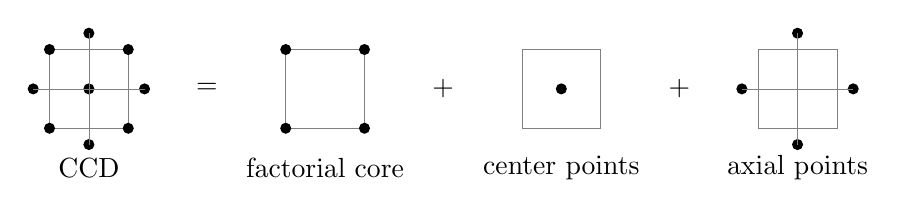
\begin{tikzpicture}
		\def\a{1.414}
		\def\u{1}
		\def\cw{4pt}
		
		\begin{scope}[scale=0.5]
			\draw [help lines] (\u,\u) -- (-\u,\u) -- (-\u,-\u) -- (\u,-\u) -- cycle;
			\fill (-\a,0) circle (\cw) (\a,0) circle (\cw) (0,-\a) circle (\cw) (0,\a) circle (\cw);
			\fill (\u,\u) circle (\cw) (-\u,\u) circle (\cw) (-\u,-\u) circle (\cw) (\u,-\u) circle (\cw);
			\fill (0,0) circle (\cw);
			\draw [help lines] (-\a,0) -- (\a,0) (0,-\a) -- (0,\a);
			\node at (0,-2) {CCD};
		\end{scope}
		\node at (1.5,0) {$=$};
		\begin{scope}[shift={(3,0)},scale=0.5]
			\draw [help lines] (\u,\u) -- (-\u,\u) -- (-\u,-\u) -- (\u,-\u) -- cycle;
			\fill (\u,\u) circle (\cw) (-\u,\u) circle (\cw) (-\u,-\u) circle (\cw) (\u,-\u) circle (\cw);
			\node at (0,-2) {factorial core};
		\end{scope}
		\node at (4.5,0) {$+$};
		\begin{scope}[shift={(6,0)},scale=0.5]
			\draw [help lines] (\u,\u) -- (-\u,\u) -- (-\u,-\u) -- (\u,-\u) -- cycle;
			\fill (0,0) circle (\cw);
			\node at (0,-2) {center points};
		\end{scope}
		\node at (7.5,0) {$+$};
		\begin{scope}[shift={(9,0)},scale=0.5]
			\draw [help lines] (\u,\u) -- (-\u,\u) -- (-\u,-\u) -- (\u,-\u) -- cycle;
			\fill (-\a,0) circle (\cw) (\a,0) circle (\cw) (0,-\a) circle (\cw) (0,\a) circle (\cw);
			\draw [help lines] (-\a,0) -- (\a,0) (0,-\a) -- (0,\a);
			\node at (0,-2) {axial points};
		\end{scope}
	\end{tikzpicture}
\end{center}

\begin{center}
	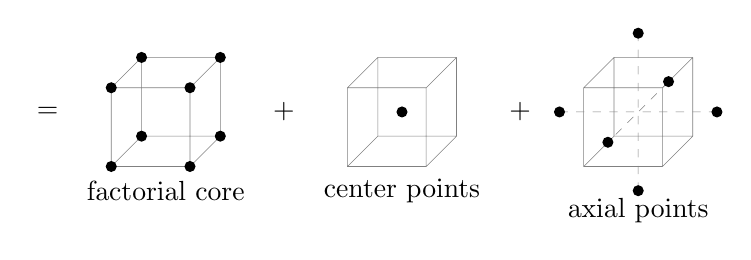
\begin{tikzpicture}
		\def\a{2}
		\def\u{1}
		\def\cw{4pt}
		\node at (1.5,0) {$=$};
		\begin{scope}[shift={(3,0)},scale=0.5]
			\draw [help lines] 
				(\u,\u,-\u) -- (-\u,\u,-\u) -- (-\u,-\u,-\u) -- (\u,-\u,-\u) -- (\u,\u,-\u)
				(\u,\u,\u) -- (-\u,\u,\u) -- (-\u,-\u,\u) -- (\u,-\u,\u) -- (\u,\u,\u)
				(\u,\u,-\u) -- (\u,\u,\u)
				(-\u,\u,-\u) -- (-\u,\u,\u)
				(-\u,-\u,-\u) -- (-\u,-\u,\u)
				(\u,-\u,-\u) -- (\u,-\u,\u);
			\fill (\u,\u,\u) circle (\cw) (-\u,\u,\u) circle (\cw) (-\u,-\u,\u) circle (\cw) (\u,-\u,\u) circle (\cw)
				  (\u,\u,-\u) circle (\cw) (-\u,\u,-\u) circle (\cw) (-\u,-\u,-\u) circle (\cw) (\u,-\u,-\u) circle (\cw);
			\node at (0,-2) {factorial core};
		\end{scope}
		\node at (4.5,0) {$+$};
		\begin{scope}[shift={(6,0)},scale=0.5]
			\draw [help lines] 
				(\u,\u,-\u) -- (-\u,\u,-\u) -- (-\u,-\u,-\u) -- (\u,-\u,-\u) -- (\u,\u,-\u)
				(\u,\u,\u) -- (-\u,\u,\u) -- (-\u,-\u,\u) -- (\u,-\u,\u) -- (\u,\u,\u)
				(\u,\u,-\u) -- (\u,\u,\u)
				(-\u,\u,-\u) -- (-\u,\u,\u)
				(-\u,-\u,-\u) -- (-\u,-\u,\u)
				(\u,-\u,-\u) -- (\u,-\u,\u);
			\fill (0,0,0) circle (\cw);
			\node at (0,-2) {center points};
		\end{scope}
		\node at (7.5,0) {$+$};
		\begin{scope}[shift={(9,0)},scale=0.5]
			\draw [help lines] 
				(\u,\u,-\u) -- (-\u,\u,-\u) -- (-\u,-\u,-\u) -- (\u,-\u,-\u) -- (\u,\u,-\u)
				(\u,\u,\u) -- (-\u,\u,\u) -- (-\u,-\u,\u) -- (\u,-\u,\u) -- (\u,\u,\u)
				(\u,\u,-\u) -- (\u,\u,\u)
				(-\u,\u,-\u) -- (-\u,\u,\u)
				(-\u,-\u,-\u) -- (-\u,-\u,\u)
				(\u,-\u,-\u) -- (\u,-\u,\u);
			\draw [help lines,dashed] (-\a,0,0) -- (\a,0,0) (0,-\a,0) -- (0,\a,0) (0,0,-\a) -- (0,0,\a);
			\fill (-\a,0,0) circle (\cw) (\a,0,0) circle (\cw) 
				  (0,-\a,0) circle (\cw) (0,\a,0) circle (\cw)
				  (0,0,-\a) circle (\cw) (0,0,\a) circle (\cw);
			\node at (0,-2.5) {axial points};
		\end{scope}
	\end{tikzpicture}
\end{center}
	
\end{frame}

\begin{frame}{Parts of the CCD}
	\begin{center}
	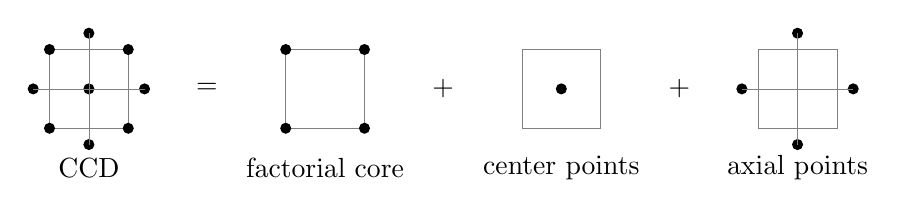
\begin{tikzpicture}
		\def\a{1.414}
		\def\u{1}
		\def\cw{4pt}
		
		\begin{scope}[scale=0.5]
			\draw [help lines] (\u,\u) -- (-\u,\u) -- (-\u,-\u) -- (\u,-\u) -- cycle;
			\fill (-\a,0) circle (\cw) (\a,0) circle (\cw) (0,-\a) circle (\cw) (0,\a) circle (\cw);
			\fill (\u,\u) circle (\cw) (-\u,\u) circle (\cw) (-\u,-\u) circle (\cw) (\u,-\u) circle (\cw);
			\fill (0,0) circle (\cw);
			\draw [help lines] (-\a,0) -- (\a,0) (0,-\a) -- (0,\a);
			\node at (0,-2) {CCD};
		\end{scope}
		\node at (1.5,0) {$=$};
		\begin{scope}[shift={(3,0)},scale=0.5]
			\draw [help lines] (\u,\u) -- (-\u,\u) -- (-\u,-\u) -- (\u,-\u) -- cycle;
			\fill (\u,\u) circle (\cw) (-\u,\u) circle (\cw) (-\u,-\u) circle (\cw) (\u,-\u) circle (\cw);
			\node at (0,-2) {factorial core};
		\end{scope}
		\node at (4.5,0) {$+$};
		\begin{scope}[shift={(6,0)},scale=0.5]
			\draw [help lines] (\u,\u) -- (-\u,\u) -- (-\u,-\u) -- (\u,-\u) -- cycle;
			\fill (0,0) circle (\cw);
			\node at (0,-2) {center points};
		\end{scope}
		\node at (7.5,0) {$+$};
		\begin{scope}[shift={(9,0)},scale=0.5]
			\draw [help lines] (\u,\u) -- (-\u,\u) -- (-\u,-\u) -- (\u,-\u) -- cycle;
			\fill (-\a,0) circle (\cw) (\a,0) circle (\cw) (0,-\a) circle (\cw) (0,\a) circle (\cw);
			\draw [help lines] (-\a,0) -- (\a,0) (0,-\a) -- (0,\a);
			\node at (0,-2) {axial points};
		\end{scope}
	\end{tikzpicture}
\end{center}

\begin{itemize}[<+->]
	\item Factorial points alone estimates the FO and TWI terms. The core must be Resolution~$\mathrm{V}$ or higher.
	\item Axial points allow estimation of the PQ terms. Without axial points we could only estimate the sum of all PQ terms.
	\item CCDs have a pair of axial runs for each factor:
		\begin{itemize}
			\item One factor is set to $\pm\alpha$
			\item All other factors are set to 0.
		\end{itemize}
	\item Center points estimate pure error and help (some) with PQ terms.
	\item To build a CCD you need to decide:
		\begin{enumerate}
			\item The size of the FF core
			\item The number of center runs
			\item The value of $\alpha$
		\end{enumerate}
	
\end{itemize}
\end{frame}

\begin{frame}{Uniform precision}

\begin{itemize}
	\item A model has \textbf{uniform precision} if the variance at design radius~1 is the same as at the center.
\end{itemize}

\onslide<2->{
	\begin{center}
		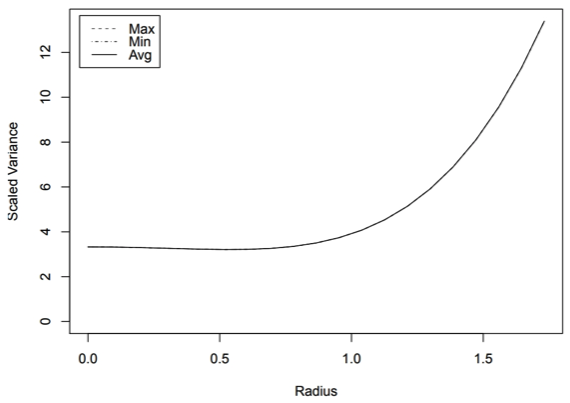
\includegraphics[width=0.5\textwidth]{figures/variance_dispersion.png}
	\end{center}
}

\begin{itemize}
	\item<3-> Choosing the correct number of center points in a CCD ensures uniform precision.
\end{itemize}
	
\end{frame}


\begin{frame}{Rotatable designs}

\begin{itemize}
	\item Models are most precise at the center of the design.
	\item<2-> Ideally, the change in precision should be independent of the \emph{direction} we move away from the center.
\end{itemize}


\onslide<3->{
	\begin{center}
		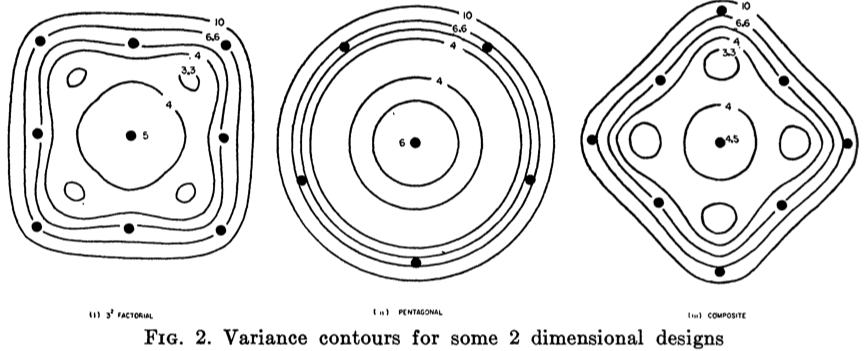
\includegraphics[width=0.5\textwidth]{figures/unequal_variance.png}
	\end{center}
	\begin{center}\tiny{Image from Box and Hunter 1957.}\end{center}
}

\begin{itemize}
	\item<4-> Designs where the variance only depends on the radius are called \textbf{rotatable designs}.
	\item<5-> A CCD with $F$ factorial points is rotatable when $\alpha=\sqrt[4]{F}$.
\end{itemize}
\end{frame}

\begin{frame}{Rotatable, uniform precision CCDs}
	\begin{tabular}{lcccccccccccc}
	  factors ($k$) & 2 & 3 & 4 & 5 & $5-1$ & 6 \\
	  \hline
	  factorial points & 4 & 8 & 16 & 32 & 16 & 64 \\
	  axial points & 4 & 6 & 8 & 10 & 10 & 12 \\
	  center points & 5 & 6 & 7 & 10 & 6 & 15 \\
	  axial distance ($\alpha$) & 1.414 & 1.682 & 2.000 & 2.378 & 2.000 & 2.828
	\end{tabular}

	\bigskip\bigskip
	\begin{tabular}{lcccccccccccc}
	  factors ($k$) & $6-1$ & 7 & $7-1$ & 8 & $8-1$ & $8-2$ \\
	  \hline
	  factorial points & 32 & 128 & 64 & 256 & 128 & 64 \\
	  axial points & 12 & 14 & 14 & 16 & 16 & 16 \\
	  center points & 9 & 21 & 14 & 28 & 20 & 13 \\
	  axial distance ($\alpha$) & 2.378 & 3.364 & 2.828 & 4.000 & 3.364 & 2.828
	\end{tabular}
\end{frame}

\begin{frame}{Factor levels in a CCD}
Each factor in the CCD will be set at five levels:
\[ -\alpha\quad-1\quad\phantom{-}0\quad\phantom{-}1\quad\phantom{-}\alpha \]
\pause
Unlike a 2-level design, the coded units in a CCD have meaning!
\end{frame}

\begin{frame}{Coding the CCD}

Let's say we're designing a combination screening of three drugs. The absolute widest concentration range we can use for drug A is $[-3.2, 1.0]$ on a $\log_{10}$-$\mu$M scale. What are the five levels assuming a full-factorial CCD?
\pause
\[ F = 2^3 = 8 \Rightarrow \alpha = \sqrt[4]{8} = 1.68 \]
\pause
\begin{align*}
\text{A} &= \text{center}(\text{A}) + \frac{\text{range}(\text{A})}{2\alpha}[\text{code}] \\
  &= -1.1 + \frac{1 - (-3.2)}{2(1.68)}[\text{code}]
\end{align*}

\pause
\begin{center}
\begin{tabular}{rccccc}
  code: & $-\alpha$ & $-1$ & $\phantom{-}0$ & $1$ & $\alpha$ \\
  $\log_{10}$-$\mu$M: & $-3.2$ & $-2.4$ & $-1.1$ & $0.2$ & $1.0$
\end{tabular}
\end{center}

\end{frame}

\end{document}
